\normalfalse \difficiletrue \tdifficilefalse
\correctionfalse

%\UPSTIidClasse{11} % 11 sup, 12 spé
%\newcommand{\UPSTIidClasse}{11}

\exer{Mouvement RR 3D  $\star\star$ \label{C1:05:08}}
\setcounter{question}{0}

\marginnote{\xpComp{DYN}{05}}%\UPSTIcompetence{B2-14}
%\UPSTIcompetence[2]{C1-05}
\index{Compétence B2-14}
\index{Compétence C1-05}
\index{PFS}
\index{Mécanisme à 2 rotations 3D}
\ifcorrection
\else
\marginnote{\textbf{Pas de corrigé pour cet exercice.}}
\fi

\ifprof
\else
Soit le mécanisme suivant. On a $\vect{AB}=H\vect{j_1}+R\vect{i_1}$ et $\vect{BC}=L\vect{i_2}$. On a $H=\SI{20}{mm}$, $r=\SI{5}{mm}$, $L=\SI{10}{mm}$. De plus :
\begin{itemize}
\item $G_1$ désigne le centre d'inertie de \textbf{1} tel que $\vect{AG_1}=H\vect{j_1}$, on note $m_1$ la masse de \textbf{1};% et $\inertie{G_1}{1}=\matinertie{A_1}{B_1}{C_1}{0}{0}{0}{\bas{1}}$; 
\item $G_2=C$ désigne le centre d'inertie de \textbf{2}, on note $m_2$ la masse de \textbf{2}.% et $\inertie{G_2}{2}=\matinertie{A_2}{B_2}{C_2}{0}{0}{0}{\bas{2}}$.
\end{itemize}

Un moteur électrique positionné entre \textbf{0} et \textbf{1} permet d'actionner le solide \textbf{1}.
Un moteur électrique positionné entre \textbf{1} et \textbf{2} permet d'actionner le solide \textbf{2}.
L'accélération de la pesanteur est donnée par $\vect{g}=-g\vect{j_0}$.

\begin{figure}[!h]
\centering
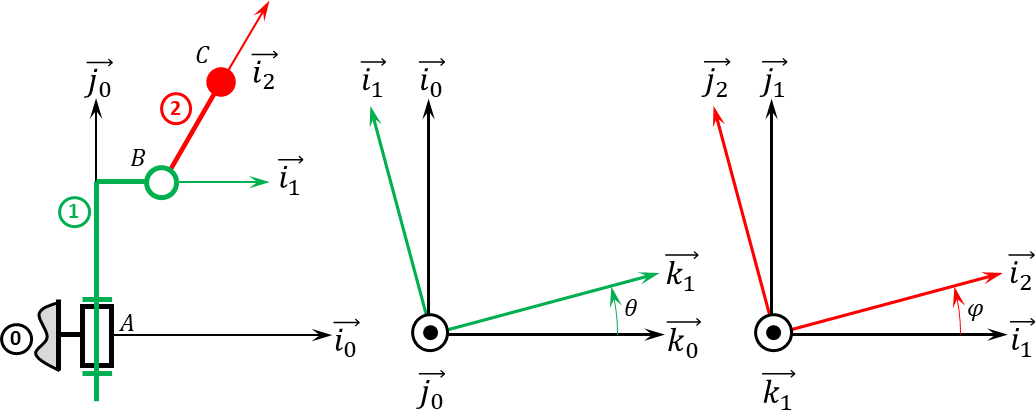
\includegraphics[width=\linewidth]{08_RR3D_01}
\end{figure}
\fi

\question{Réaliser le graphe d'analyse en faisant apparaître l'ensemble des actions mécaniques.}
\ifprof
\else
\fi

\question{Proposer une démarche permettant de déterminer les loi de mouvement de \textbf{1} et de \textbf{2} par rapport à $\rep{0}$.}
\ifprof
\else
\fi

\ifcolle
\question{Mettre en \oe{}uvre cette démarche.}
\ifprof
\else
\fi
\else
\fi

\ifprof
\else
\marginnote{Corrigé voir \ref{C1:05:08}.}
\fi